\chapter{Results and Discussions}
\label{chap:results}

In this chapter, we gather results from the different experiments we want to run. Subsequentially, we discuss the results and look at current limitations. Finally, we delve deeper into whether or not \Gls{julia} has proven to be a satisfactory language for our case. \\


Apples in my asshole \cite{projthesis}
a \cite{claerbout1991scrutiny}
a \cite{landes1951scrutiny}
a \cite{omar2013machine}
a \cite{wei2022lstmautoencoder}
a \cite{julia}
a \cite{apSensing2019railwaydas}
a \cite{DBLP:journals/corr/SrivastavaMS15}
a \cite{2011ndongsigprocandet}
a \cite{doi:10.1137/141000671}
a \cite{bioengineering10040405}
a \cite{maulik2020recurrent}



\section{Results Setup}

\begin{equation}
    TPR(TruePositiveRate/Recall) = \frac{TP}{TP + FN}
\end{equation}

\begin{equation}
    FPR(FalsePositiveRate/Recall) = \frac{FP}{FP + TN}
\end{equation}

\begin{equation}
    Precision = \frac{TP}{TP + FP}
\end{equation}

\begin{equation}
    F1 - score = 2 x (\frac{Precision \cdot Recall}{Precision + Recall})
\end{equation}

\begin{equation}
    Accuracy = \frac{TP + TN}{TP + TN + FP + FN}
\end{equation}


\begin{tikzpicture}[h]
\centering
  \begin{axis}[ 
    xlabel=$x$,
    ylabel={$relu$},
    xmin=-3, ymax=3,
    ymin=-2, ymax=3,
    grid=both,
  ] 
    \addplot[red, domain=-3:3] {max(0, x)}; 
    
  \end{axis}
\end{tikzpicture}

\begin{table}[h]
\centering
\begin{tabular}{|ll|ll|}
\hline
\multicolumn{2}{|c|}{\multirow{2}{*}{\textbf{Total Population}}} & \multicolumn{2}{c|}{Predictions}      \\ \cline{3-4} 
\multicolumn{2}{|c|}{}                                           & \multicolumn{1}{l|}{Normal} & Anomaly \\ \hline
\multicolumn{1}{|l|}{\multirow{2}{*}{Actual}}      & Normal      & \multicolumn{1}{l|}{TN}     & FP      \\ \cline{2-4} 
\multicolumn{1}{|l|}{}                             & Anomaly     & \multicolumn{1}{l|}{FN}     & TP      \\ \hline
\end{tabular}
\label{tab:confmat}
\caption{Confusion matrix}
\end{table}

\begin{table}[h]
\centering
\begin{tabular}{|l|l|}
\hline
\textbf{Unit} & \textbf{Desc}         \\ \hline
Os            & Ubuntu Linux          \\ \hline
Processor     & Intel i9-9940X @ 4GHz \\ \hline
Ram           & 126GB                 \\ \hline
GPU           & NVIDIA RTX 2080TI     \\ \hline
VRAM          & 11GB                  \\ \hline
Gpu Cores     & 4352                  \\ \hline
Packages      & Flux 2.1., CUDA       \\ \hline
\end{tabular}
\label{tab:specs}
\caption{Specs for our machine running our code}
\end{table}



\subsubsection{Experiment 1: This is how we do it}

NOW

\begin{figure}
  \begin{subfigure}[t]{.5\textwidth}
    \centering
    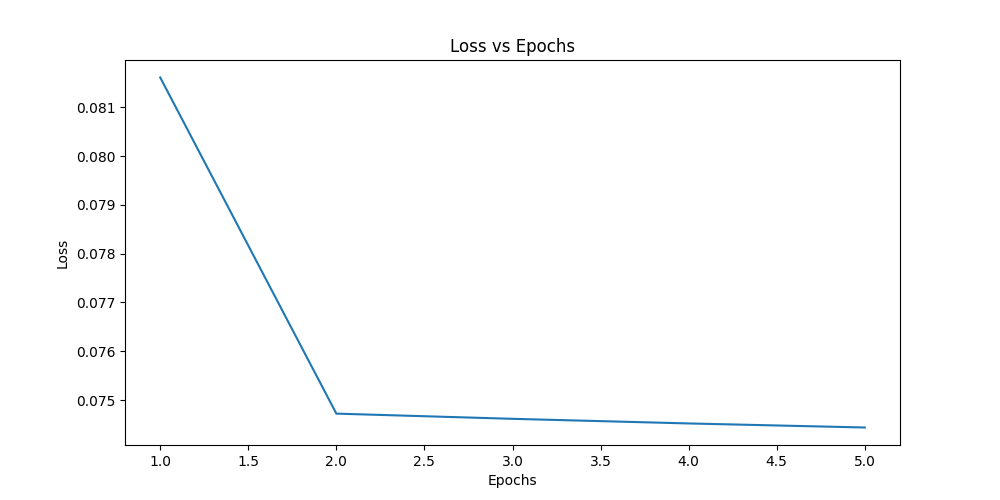
\includegraphics[width=\linewidth]{figures/loss.png}
    \caption{AE}
  \end{subfigure}
  \hfill
  \begin{subfigure}[t]{.5\textwidth}
    \centering
    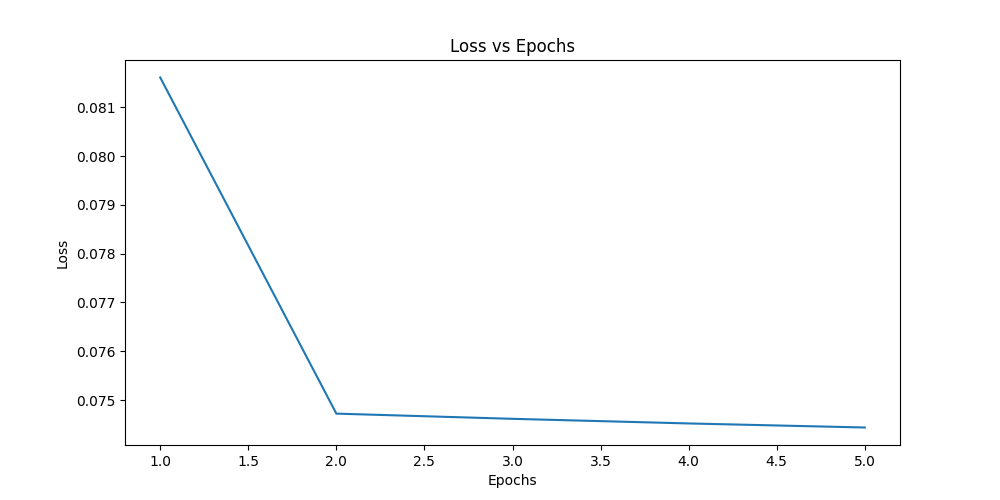
\includegraphics[width=\linewidth]{figures/loss.png}
    \caption{CNN AE}
  \end{subfigure}

  \medskip

  \begin{subfigure}[t]{.5\textwidth}
    \centering
    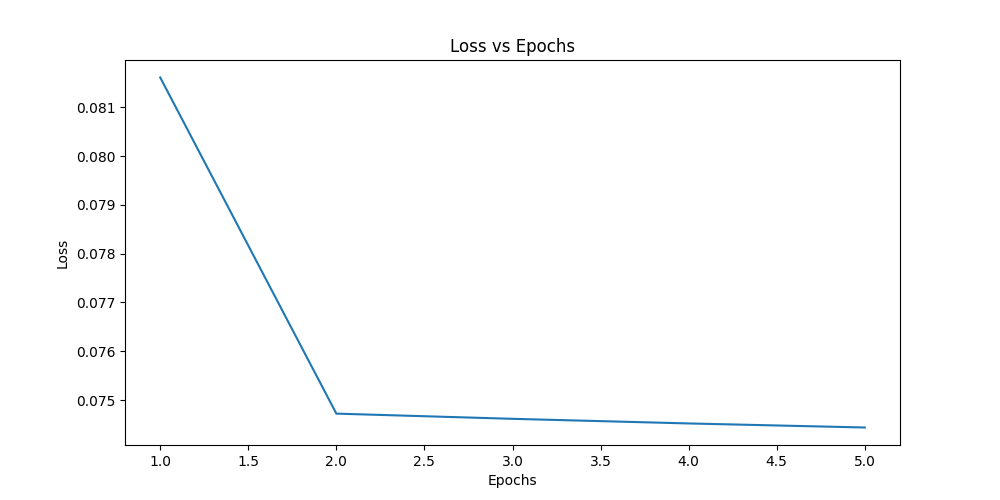
\includegraphics[width=\linewidth]{figures/loss.png}
    \caption{VAE}
  \end{subfigure}
  \hfill
  \begin{subfigure}[t]{.5\textwidth}
    \centering
    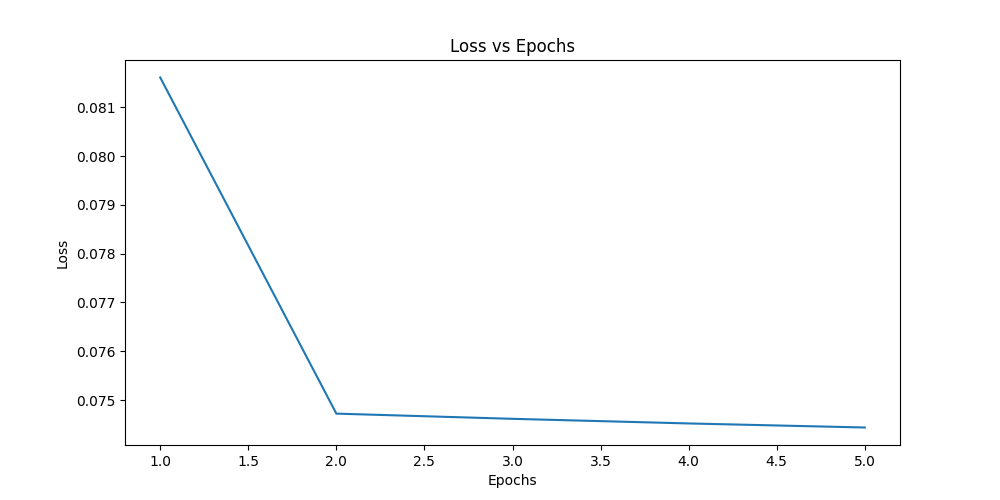
\includegraphics[width=\linewidth]{figures/loss.png}
    \caption{Beta VAE}
  \end{subfigure}
    \caption{Losses for all models}
\end{figure}
\section{Discussion}
\label{chap:discussion}

\subsection{Judas}

When we first started working on a library for das processing 

FINE GRAINED APPROACH .. \\

API Design and CGF. \\ 

\textbf{JU} \\ 

\textbf{JU} \\ 

\textbf{JU} \\ 

\subsection{TinyDAS}

aksdflkfsdjlkjsfd. \\ 
a:KLSDj.

\subsection{Modularity in Data Science}

api design for data science has for far long enough been overlooked. Full AI models are regularly being comprised in a single file, with only a argument parser to make sure python can run the script. We instead wanted to seperate between the different aspects of the AI part of the code. The models, engine and hyperparameters can all easily be split into multiple files, but yet this is not common. The advantage we gain by splitting up this module, is easier ways of debugging, as well as to more easily reuse only the sections of the code that we're interested in. Training and Inference are by default split in their own files, since we don't actually want those two run after each other. The training of the neural net should only happen when needed, inference is the mode we'd actually like to test against and return the answers about loss and so on 


\subsection{Interpretibility}
One major question we wanted to tackle is regarding interpretibility. Is this achieved, or do we still have a long way to go?

\subsection{Did we reach our goals?}

\section{Limitations}

Working on Judas with \acrshort{das} data has proven very meaningful. \\\

There are still plenty of undiscovered methods on this kind of data. As mentioned in \cite{MALEKI2021107443}, "Anomaly detection in unlabelled Big Data is difficult and costly". We've seen this occur even after multiple different rounds of resampling, channel decimation, and so on. 
\section*{Reflections on Julia}
\label{sec:juliaref}

Since the very first day of this project, we've been using Julia quite rigorously. Some may argue that C and Python would be more efficient due to their extensive ecosystems and documentations. They are also more or less the \textit{de-facto standard} programming languages for their respective fields, \acrshort{hpc} and \acrshort{ai}. Additionally, members of \acrshort{cgf} are more accustomed to these languages, so why Julia? \\

Besides what's already been mentioned, we wanted to give our thoughts on developing in Julia. Before getting started with Julia as the target language of our program, we made sure it had all the different packages we would need. For \acrshort{ai} and \acrshort{ml} packages, we were pleasantly surprised to find multiple options that all perform well. Bindings to similar packages in Python could also easily be found. We opted for Flux, and with its native integration with CUDA, no extra work had to be done to make use of \acrshort{gpu}s to speed up the computation of our models.

Next to this comes the builtin \texttt{@inbounds} macro, which turns of the boundary checker when accessing memory, speeding up computations in a short matter of time. Not only this, but all the different macros in Julia were pleasant to work with. \texttt{time}, \texttt{btime}, \texttt{profile}, \texttt{cuda}, \texttt{btime}, \texttt{simd} all help imensly when creating programs, without the need for writing loops or custom instructions. Just simply knowing how and where to place macros cleans up the code, and not only increases the developer experience, but also standardizes code between codebases without having to rewrite all from scratch. Just simply running and launcing cudakernels as in \ref{app:jlvsc} shows how easy it is to setup and run CUDA kernels as long as the \texttt{CUDA.jl} package is installed. \\

A majority of new languages and compilers comes with a version multiplexer, examples being \texttt{rustup}, \texttt{zigup}. These are not built retrospectively, as is the case for \texttt{sdkman} for Java, but before. Managing dependencies and packages, maintaining larger programs and so on becomes a lot easier with both a version multiplexer and a productive package manager. C has never had a standard way of dealing with packages, and this has inspired future languages to extend their ecosystems to include this alongside the compiler and standard library. Python has \texttt{PyPI}, but with many different programs to deal with versioning and packages. Some of these are venv, \texttt{Anaconda} and \texttt{Poetry}. Just simply installing and setting up projects in these languages seem to be harder than it actually have to be, and Julia proves this. \\ 

Enabling multiple processors or threads comes down to simply specifying a flag when running \texttt{-p} or \texttt{-t} respectively. The language has these kinds of computing built into the standard library, no need to install third party dependencies. 

When it comes to AI, Python has stayed supreme as the \textit{de-facto standard} for implementing and testing models. Tensorflow, Pytorch and recently Tinygrad are all highly optimized frameworks for working with ML, with thousands of articles, papers and learning materials written about them. Comparatively, Julias \texttt{Flux.jl} is way younger, but offers in our opinion, easier GPU toggling, model design and overall a smoother experience for . The docs of \texttt{Flux.jl} takes one through the entire code base, and after reviewing models on \cite{https://github.com/FluxML/model-zoo}, it's easy to figure out how to setup, train and save models.

Julia excels when it comes to scientific computations. Not only does the support of unicode symbols make it easier to translate white papers to code, but Julias syntax and its compilation makes for an incredible developer experience, as well as increased performance. In the appendix, one can see an example of plotting in Julia, and how intuitive it can be, compared to other languages.






Although Julia has shown to have many strengths, there is no thing such as a perfect programming language. Julias' main weaknesses besides a far younger ecosystem compared to its alternatives, is its lack of documentation. 

Another potential drawback is the relatively young ecosystem for \acrshort{ai} or \acrshort{ml} programmming that exits compared to Python. As mentioned in \ref{chap:back}, Julia has bindings for Tensorflow, yet still Flux is preferred in most cases. Although it seems to have all functions necessary for computations, some of its functions are not as optimized as they can be. As discussed in \cite{projthesis}, \lstinline|relu| was not optimized until the end of last year. These kinds of optimizations, be it trivial or not, will impact larger programs on a significat level, so we might want to benchmark certain functions to see if they may be optimized futher. However, this is also a great aspect of Julia. Due to how Flux is engineered, modifying or adding to the source code is still the way to go when looking at newer models


Conclusions on personal use 

